\chapter{Estado del arte}
\label{ch:sota}

En el siguiente capítulo pasaremos explicar qué es la esteganografía digital junto con una breve introducción a la herramienta Stegosploit. Después, pasaremos a ver brevemente los usos del Deep Learning en la esteganografía de forma general y, por último, mencionaremos los artículos que conforman el estado del arte del proyecto para poder hacer una comparativa tanto de los modelos como de las métricas utilizadas y tener una base sobre la que movernos durante la implementación del mismo, la cual veremos más adelante.

\section{¿Qué es la esteganografía?}

La esteganografía es el arte de ocultar información a simple vista dentro, o por encima, de algo que no es secreto (\cite{esteganografia-digital}). Por ejemplo, un documento de texto, un cuadro, una grabación... Sin embargo, esto no es nada nuevo: según la historia, han habido antecedentes que han podido marcar sucesos tan importantes como la Segunda Guerra Mundial, tal y como podemos ver a continuación.%cita

\subsection{Un poco de historia}

Durante la Primera Guerra Mundial se utilizó tinta invisible como aplicación de esta técnica. Durante la Segunda Guerra Mundial también se llegó a utilizar un método muy interesante: los \textbf{micropuntos}. Los micropuntos, básicamente, eran fotografías del tamaño de una página reducidas hasta ocupar un punto de 1 mm de diámetro y, para ocultarlos, se pegaban sobre un punto del texto que los encubría (\cite{cera-micropuntos}). %cita

\section{Esteganografía digital}

Con la modernización de la sociedad en cuanto a tecnología y computación se refiere, aparecieron diversas aplicaciones de esta técnica con las que se consiguió un nivel de sofisticación y detalle en la técnica adecuado a la época: ahora no sólo era mucho más fácil realizar el escondite del mensaje, también era más complicado detectarlo (\cite{esteganografia-digital}). %cita 

A continuación mencionaremos de forma superficial algunas técnicas de esteganografía digital para poner en contexto la base sobre la que se va a realizar el trabajo:

\subsection{Clasificación tradicional}
\label{sec:trad}

Este tipo de clasificación se basa en cómo se ocultan los datos. A continuación vamos a ver algunas de las técnicas que se comprenden dentro de esta rama:

\subsubsection{Técnicas basadas en la inserción (Insertion-Based)}

Estas técnicas trabajan con la inserción de bloques de datos dentro de un archivo publicable. El dato es insertado en el mismo punto del archivo. Se suelen ocultar en las partes redundantes de un archivo, de forma que el bloque de datos puede estar dividido en varias secciones, haciendo su detección muy difícil (\cite{esteganografia-digital}).%cita

Un ejemplo de uso muy bueno para esta técnica es insertar en los \ac{LSB} de un archivo de 8 ó 16 bits. Lo que se hace es codificar el mensaje en binario e introducirlo dentro de los bits 0, 1, 2 y, tal vez, 3. De esta forma, al ser una de las partes más redundantes de información del archivo, el usuario no es consciente de que ha sido modificado, y por lo tanto puede interactuar con el archivo sin saber que puede haber un mensaje o incluso un malware en su interior que se esté ejecutando.

\subsubsection{Técnicas basadas en algoritmos (Algorithmic-Based)} 

Estas técnicas utilizan alguna clase de algoritmo para decidir dónde se debería ocultar un mensaje dentro de un archivo de datos: es por ello que el bloque de datos no se inserta siempre en el mismo punto, puede estar tanto en las partes más redundantes y olvidadas como en las más importantes... Lo cual es un problema, ya que si no se efectúa bien el algoritmo la ocultación de datos sería fácilmente detectable si se comparan el archivo original con el modificado (\cite{esteganografia-digital}). %cita

El quid de la cuestión de estas técnicas reside en utilizar un algoritmo idóneo para cada tipo de archivo. Optimizando el espacio del archivo con un buen algoritmo, los resultados para la ocultación serán idóneos.

\subsubsection{Técnicas basadas en gramática (Grammar-Based)}

Existe una gran diferencia entre estas técnicas y las anteriores: para las dos primeras se utiliza siempre un archivo que será el que encubra el mensaje... Sin embargo, para estas técnicas se genera un archivo desde cero a partir de los datos a ocultar, basándose en una gramática predefinida (\cite{esteganografia-digital}). %cita

\subsection{Clasificación moderna}

A diferencia de \ref{sec:trad}, esta clasificación se basa en cómo y dónde se ocultan los datos. Es idónea para representar las técnicas desarrolladas en la esteganografía moderna.

\subsubsection{Técnicas basadas en la inserción (Insertion-Based)}

En esencia, se trata de técnicas cuyo objetivo es ocultar datos insertándolos en un archivo sin afectar a su representación, aunque se aumente su tamaño.

Lo bueno de estas técnicas es que se pueden introducir datos en el archivo sin afectar ni modificar el contenido existente. Lo malo es el incremento de tamaño, lo cual es un claro indicador de que se han introducido datos añadidos al archivo.

\subsubsection{Técnicas basadas en la sustitución (Substitution-Based)}

Estas técnicas se basan en sustituir partes del archivo encubridor por los datos a ocultar. De esta forma el tamaño del archivo no varía y, a priori, podría parecer un archivo normal y corriente.

No obstante, es importante aclarar que la sustitución de datos no puede realizarse en cualquier zona del archivo: se corre el riesgo de que al modificarlo, haya partes que queden inservibles o visualmente defectuosas. La clave es encontrar zonas redundantes del archivo y modificarlas para que no se dé ningún impacto.

Otro factor que hay que tener en cuenta es la cantidad de datos que se pueden ocultar en el archivo hasta que éste finalmente no pueda ejecutarse correctamente. En general es una técnica muy buena siempre y cuando se cumplan estas reglas.

\subsubsection{Técnicas de generación (Generation-Based)}

De la misma forma que hemos visto en las técnicas de \ref{sec:trad}, éstas tienen una principal diferencia que cabe destacar: el archivo (o los datos) a ocultar es utilizado para crear el archivo definitivo.

De esta forma, si se consigue únicamente este archivo no debería haber problemas para que el usuario no detecte el mensaje oculto. Si se consigue el archivo original y se compara con el que tiene los datos ocultos se verá que tiene una composición binaria diferente, y la detección esteganográfica será más complicada de realizar.

\subsection{Stegosploit}

Hemos visto qué clase de técnicas existen para ocultar información en archivos sin que ésta se detecte. No obstante, dentro de las atribuciones de este trabajo nos centraremos en sólo una de ellas, la de sustitución, que es en la que se basa la herramienta que vamos a utilizar para introducir malware en imágenes y sobre la que pretendemos resolver este problema: \textbf{Stegosploit} (\cite{stegosploit}). %cita

Stegosploit es una herramienta creada por el experto en seguridad Saumil Shah (\cite{saumil-shah}) cuyo objetivo es cifrar exploits ``Drive-By Browser'' en imágenes usando esteganografía. De forma resumida, la herramienta cifra los exploits en imágenes JPG y PNG; tras ello, la imagen resultante se fusiona con un HTML con un decodificador en Javascript formando así un \textbf{políglota}: el políglota parece una imagen normal a simple vista, pero se decodifica y se activa en el navegador de la víctima (\cite{stegosploit}). %cita %cita

En el siguiente capítulo, explicaremos en detalle el proceso de encriptado de la herramienta.

\section{Deep Learning para esteganografía en imágenes}

La tecnología Deep Learning se puede usar en una gran cantidad de aplicaciones de distinta índole. Sin embargo, en este proyecto nos vamos a centrar en lo que a esteganografía en imágenes se refiere.

Como tal, no hay una serie de trabajos realizados sobre Deep Learning que sirvan para detectar esteganografía en imágenes, y mucho menos uno en concreto que se centre en los políglotas de Stegosploit. No obstante, tras realizar la búsqueda de artículos académicos, hemos podido comprobar que la \textbf{clasificación de imágenes} es un método muy acertado (no tan eficaz en Machine Learning como cabría esperar con Deep Learning, pero igualmente es una solución adecuada al problema que nos atañe).

Los trabajos que a continuación pasamos a explicar se basan en métodos de Machine Learning, aunque con diferentes enfoques y aplicaciones. 

\section{Uso de Machine Learning para detectar imágenes con políglotas maliciosos}

El objetivo de este proyecto no era otro que hacer una herramienta de Machine Learning para detectar políglotas maliciosos en imágenes (\cite{ml-stenography-shawat}). A continuación, pasaremos a listar y explicar de forma resumida el proceso que realizaron los autores para ello. %cita

Este estudio ha sido realizado tomando como base el artículo de Stegosploit del que también nos hemos servido para este trabajo (\cite{stegosploit}). %cita

\subsection{Estudiar y construir ataques XSS y CSRF}

En esta fase se procede a ver cómo se puede distribuir a las víctimas las imágenes con el código malicioso en su interior. Para ello, se estudiaron diferentes tipos de ataques sobre los que poder hacerlo, de tal forma que la víctima no se diera cuenta. A continuación, vamos a ver de manera muy superficial en qué consisten:

\subsubsection{Reflected XSS}

Este ataque se basa en la posibilidad de que un atacante modifique una URL de una aplicación con código malicioso. Si esta URL modificada es enviada a un usuario porque éste, por ejemplo, la solicita; el código malicioso se ejecutará en el navegador de la víctima, dentro de la sesión que tenga abierta en la aplicación (\cite{reflected-xss}). %cita

\subsubsection{DOM XSS}

Este ataque, no dista demasiado del anterior, sin embargo tiene otro enfoque: El atacante crea un payload, por ejemplo en la URL de la aplicación, que se ejecuta en el navegador de la víctima debido a una modificación del entorno del DOM usado en el código original de la misma. Así el cliente ejecuta el código del atacante de manera inesperada. De este modo, la página web como tal no cambia, pero en la parte de la víctima, el código contenido en la página se ejecuta de forma diferente por los cambios efectuados en el DOM (\cite{dom-xss}).

Dicho de otra forma, si por ejemplo se crea un payload en la URL y ésta se envía a la víctima, se modifica el entorno del DOM, el cual detecta el payload en la URL y se ejecuta como un objeto más del código de la aplicación.

Como se puede ver, el resultado es el mismo que en el ataque anterior, no obstante recorre otro camino para conseguirlo. %cita

\subsubsection{Persistent XSS}

Para realizar este ataque hay que inyectar código directamente en un servidor objetivo. De esta forma, cada vez que el usuario pida la información de dicho servidor, obtendrá el código introducido por el atacante. Los servidores objetivo para este tipo de ataques suelen ser bases de datos, un foro de mensajes, un registro de visitas, etc (\cite{persistent-xss}). %cita

\subsubsection{CSRF}

Este tipo de ataques fuerzan a un usuario a ejecutar acciones no deseadas en una aplicación web en la que ya están autenticados. Mediante un email o un chat, un atacante puede enviar a la víctima un enlace para engañarla y ejecutar acciones de la elección del atacante (\cite{csrf}). %cita

\subsection{Creación de políglotas}

Para crear los políglotas con los que explotar el ataque nos basaremos completamente en Stegosploit (\cite{stegosploit}).

Todo comienza cifrando el código malicioso en los bits de una imagen. Después pasamos a insertar un decodificador en la cabecera de la imagen para crear IMAJS, formando así un políglota. Por último, nos servimos de alguno de los ataques de la fase anterior para atacar a un servidor web con el políglota como recurso.

\subsection{Uso de Machine Learning para detectar imágenes con políglotas maliciosos}

A continuación, pasamos a explicar la última parte de este modelo:

\begin{figure}[H]
  \centering
  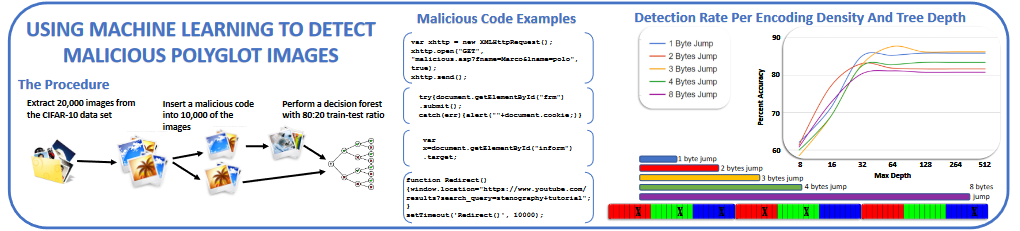
\includegraphics[width=18cm, height=6cm]{Figuras/Estado\_del\_Arte/Shawat-3.png}
  \label{fig:shawat-3}
  \caption{Detección de políglotas (\cite{ml-stenography-shawat})}
\end{figure}

Comenzamos extrayendo 20.000 imágenes del dataset \textbf{CIFAR-10} (\cite{cifar10}) para después insertar en la mitad de ellas código malicioso mediante Stegosploit (\cite{stegosploit}). %cita #cita

Ahora se utiliza el método de árboles de decisión para el dataset completo (80\% de train y 20\% de test). Los árboles de decisión son un método de Machine Learning usado en problemas de regresión y clasificación; el objetivo es crear un modelo que prediga el valor de una variable aprendiendo mediante simples reglas de decisión inferidas por los datos de entrada (\cite{decision-trees}). %cita

Los resultados finales vienen representados según una gráfica en la que se utiliza la siguiente métrica: La velocidad de detección de código por densidad de cifrado y profundidad del árbol.

Con esta métrica se quiere comprobar a qué velocidad detecta este método el código cifrado en las imágenes dependiendo de la densidad del cifrado y de la profundidad del árbol; es decir, dependiendo de en cuántos bytes se han modificado los bits y con qué distancia están separados éstos entre sí, y dependiendo de la cantidad de ramificaciones del árbol de decisión según las reglas que ha ido adoptando.

\section{Stegomalware}

Uno de los trabajos más recientes en cuanto a detección de malware en imágenes se refiere nos presenta una revisión de los modelos de detección usados durante los últimos tiempos junto con una propuesta de modelo original generada con la base de los mismos (\cite{stegomalware}). %cita

Dentro del trabajo se extiende una alta gama de contenidos como las herramientas usadas para insertar malware en imágenes mediante esteganografía, el tipo de formato de archivos usados para ello, los algoritmos de esteganografía en imágenes... Para este apartado de la memoria sólo trataremos las técnicas de estegoanálisis usadas para la detección de esteganografía en imágenes, el modelo de detección propuesto por los autores y las métricas usadas durante los experimentos.

\subsection{Técnicas de estegoanálisis}

El estegoanálisis es el acto de determinar si hay datos ocultos en el medio en el que supuestamente están y el algoritmo esteganográfico usado para introducirlo (además de extraer los datos si los hubiere). A continuación vamos a pasar a explicar cronológicamente, y de forma resumida, el estado del arte de estas técnicas:

\subsubsection{Soluciones de modelos de estegoanálisis enriquecidos y de características basadas en el dominio de imágenes}

Durante las dos últimas décadas se han ido desarrollando diferentes soluciones para abordar el problema de la esteganografía desde este enfoque. Desde un principio la investigación se concentró en detecciones basadas en Machine Learning y en características de la imagen, seguidas por modelos enriquecidos y por soluciones basadas en clasificadores de conjunto. 

Algunos de los métodos de estegoanálisis como \textbf{PHARM} (\cite{pharm}) y \textbf{GFR} (\cite{gfr}) siguieron siendo efectivos antes de la aparición del Deep Learning. Sin embargo, en el momento en el que surge esta tecnología, la investigación de estegoanálisis en imágenes convencional se reduce, y es más difícil hacer contribuciones científicas en este ámbito mejorando los métodos anteriormente mencionados. Con el Deep Learning se da un salto de calidad, y la rapidez en el desarrollo de esta rama es mucho más alta en comparación (incluyendo el estegoanálisis). %cita #cita

Aun con la aparición de esta nueva tecnología, el rendimiento ofrecido por estos métodos sirvió como pie de apoyo para mejorar las soluciones que posteriormente aparecerían gracias al Deep Learning. Las soluciones de este apartado se evaluaron y compararon con otras usando métricas de error y de precisión de detección. Los investigadores, además, usaron algoritmos de esteganografía estándar como \textbf{HUGO} (\cite{hugo}), \textbf{UNIWARD} (\cite{uniward}) o \textbf{WOW} (\cite{wow}) para evaluar la efectividad de las soluciones de estegoanálisis.%#cita #cita #cita

Los resultados de la evaluación iban mejorando cada año y, consecuentemente, aparecieron más soluciones por probar. Hasta 2015, año de aparición de Deep Learning, técnicas como GRF o PHARM fueron de lo mejor que hubo. No obstante, ninguno de estos modelos fue evaluado según la detección de malware: es en este punto donde el Deep Learning toma partida en el estegoanálisis.

\subsubsection{Modelos de Deep Learning para el estegoanálisis de imágenes}

Dentro de la lectura de este trabajo, se proponen una buena cantidad de soluciones de Deep Learning para conseguir la tan ansiada detección de esteganografía en imágenes con unos resultados muy prometedores. Las soluciones principalmente se enfocan en proponer cambios en la capa de preprocesado, en la función de activación, en la disposición de las capas convolucionales y en la fusión de bloques; y en la clasificación lineal para capturar elementos esteganográficos.

Al experimentar con las soluciones se ha sacado en claro que hay varios modelos como \textbf{SR-Net} o \textbf{Zhu-Net}, que han conseguido muy buenos resultados en lo que a errores y precisión de detección se refiere. De hecho, estos modelos pueden llegar a ser una referencia para hacer comparativas en el futuro cuando surjan nuevas contribuciones.

Sin embargo, y a pesar de que el campo de Deep Learning ofrece muchas más posibilidades y caminos a tomar para seguir desarrollándose, todavía no hay trabajos que utilicen esta tecnología para la detección de malware... A continuación veremos la propuesta del modelo de los autores para abarcar un nuevo enfoque en la tecnología de Deep Learning.

\subsection{Modelo de detección de stegomalware}

El modelo está pensado para aplicarse dentro del ámbito de la empresa y, dependiendo del tamaño de ésta, de la frecuencia de imágenes con esteganografía cotejadas por la misma, del número de archivos multimedia recibidos por la organización y de las operaciones de negocio de ésta; la estructura del modelo variará.

En general, el proceso es como se ve en la imagen, en el contexto de una aplicación de una empresa:

\begin{figure}[H]
  \centering
  \includegraphics[width=0.60\linewidth]{Figuras/Estado\_del\_Arte/Stegomalware/Modelo\_Autores.png}
  \label{fig:modelo-autores}
  \caption{Modelo de los autores (\cite{stegomalware})}
\end{figure}

\begin{itemize}
\item Un empleado informa de un archivo de imagen sospechoso en un correo de phishing (por ejemplo), entonces la imagen se sube a una ubicación de almacenamiento estándar, la cual está aislada del resto de la infraestructura de la aplicación por motivos obvios. Adicionalmente, el equipo de seguridad podrá subir, si precisa, el archivo para analizarlo.
\item El archivo puede ser escaneado debido a la posibilidad de tener un posible malware, además de poder determinarse cuán malicioso es mediante herramientas de detección de firma (\cite{signature-based-detection}). Estas herramientas indican si la amenaza es conocida o no (si no es conocida, se le pone un identificador para el futuro). %cita
\item Si efectivamente el archivo tiene un malware, marcamos la imagen y realizamos acciones preventivas como aislar la máquina infectada o actualizar el hash de la firma del malware de la imagen en las políticas de seguridad de la organización para bloquear el malware y detener la infección de la red.
\item Si por el contrario, no se identifica el archivo como malicioso dentro de este sistema de detección preliminar lo pasamos al siguiente paso: \textbf{Identificar el tipo de archivo que es y el formato que tiene}.
\item Actualmente existen muchos tipos de formato en los archivos multimedia, y uno de los principales retos es identificar el malware en estas condiciones en donde el archivo puede ser de cualquier tipo.
\item Si el archivo no es multimedia se seguirá el procedimiento normal de enviarlo a la herramienta anti-malware para su análisis.
\item Si por el contrario, sí se identifica como archivo multimedia, debemos realizar un análisis estructural y estadístico del archivo para la detección del malware. El análisis estructural incluye: cambios en la marca de tiempo y en las fechas, propiedades del archivo inusuales como el tamaño del archivo, el checksum y la modificación del contenido, anomalías en el contenido de la cabecera \textbf{Exif} (\cite{exif-header})... Para ello, usamos las herramientas de código abierto \textbf{StegSpy} (\cite{stegspy}) y \textbf{stego-toolkit} (\cite{stego-toolkit}). %cita #cita #cita
\item Si hubiera alguna propiedad anómala detectada, se marcaría el archivo como sospechoso para realizar más análisis.
\item Por otro lado, tenemos el análisis estadístico del archivo. Este es realizado para encontrar más pruebas para saber cuán malicioso es el archivo. Las propiedades estadísticas pueden incluir histogramas de bytes y n-gramas del archivo, los cambios de patrón en los píxeles de la imagen o en los frames de un vídeo y los cambios en los bit menos significativos de las imágenes. Las herramientas usadas en este tipo de análisis para esta propuesta son: \textbf{StegExpose} (\cite{stegexpose}) y \textbf{Stegdetect} (\cite{stegdetect}). %cita #cita
\item La respuesta colectiva de los resultados de ambos análisis se combinan y se evalúa de nuevo cuán malicioso es el archivo, o si es sospechoso de tener un malware en su interior.
\item Si el archivo se indica como sospechoso o malicioso, se envía a un entorno de \textbf{Cuckoo Sandbox} (\cite{cuckoo-sandbox}) para aplicar un análisis de malware dinámico e identificar las características de comportamiento del archivo.%#cita
\item Hay una alta probabilidad de que el contenido malicioso oculto en el archivo pueda ser extraído y ejecutado como resultado de unas instrucciones de código embebido. Por ejemplo, un código de shell embebido en el archivo de imagen puede ser ejecutado e intentar conectarse a un servidor remoto para ejecutar comandos maliciosos y exfiltrar datos de la organización.
\item De este modo, basándonos en el comportamiento del malware, tenemos que tomar acciones preventivas en el entorno si el archivo acaba siendo finalmente malicioso.
\item Las acciones preventivas pasan por poder actualizar, de nuevo, la firma del malware para los indicadores de compromiso como direcciones IP, dominios, y otras firmas de código hexadecimal para la detección de malware en el entorno de la infraestructura.
\item Sin embargo, si el archivo se comporta con normalidad durante el análisis dinámico, podemos ignorar el archivo para futuras acciones y podemos seguir la pista del mismo por si se diese el caso de que fuese un falso positivo en el futuro.
\end{itemize}

A continuación, pasaremos a revisar las métricas usadas.

\subsection{Métricas}

En esta revisión se han utilizado numerosas métricas para medir las técnicas de esteganografía en imágenes bajo un baremo apropiado para éstas. De forma resumida, vamos a pasar a explicarlas para tomarlas como referencia en nuestro trabajo, a pesar de que nuestro objetivo es diferente al de esta revisión.

\subsubsection{PSNR}

Esta métrica es muy útil para evaluar la calidad de la imagen. Se puede usar para medir la distorsión entre imágenes con esteganografía e imágenes sin ésta. Se sirve de la función \ac{MSE} (o Error Cuadrático Medio), tal y como viene en la siguiente figura (\cite{mse-ssim}): %cita

\begin{figure}[H]
  \centering
  \begin{subfigure}[H]{0.45\linewidth}
  \centering
  	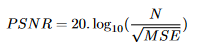
\includegraphics[width=0.60\linewidth]{Figuras/Estado\_del\_Arte/Stegomalware/PSNR.png}
  	\label{fig:PSNR}
  	\caption{PSNR}
  \end{subfigure}
  \begin{subfigure}[H]{0.45\linewidth}
  \centering
  	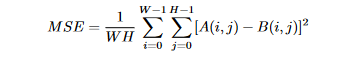
\includegraphics[width=0.80\linewidth]{Figuras/Estado\_del\_Arte/Stegomalware/MSE.png}
  	\label{fig:MSE}
  	\caption{MSE}
  \end{subfigure}
  \caption{Ecuaciones de PSNR (\cite{stegomalware})}
\end{figure}

Donde la \textit{N} es la máxima diferencia entre píxeles en una imagen. Si el \ac{MSE} es alto en un algoritmo de esteganografía, es más complicado realizar el estegoanálisis que en un algoritmo con el \ac{MSE} bajo. Con la métrica \ac{PSNR} pasa lo mismo: si tiene un valor alto, es más complejo saber si una imagen tiene o no datos introducidos por esteganografía. Dicho de otra forma, si el \ac{PSNR} está por encima de los 30 dB, es muy difícil para el ojo humano saber distinguir entre una imagen con esteganografía y otra sin ella.

\subsubsection{SSIM}

La métrica \ac{SSIM} se utiliza para la medida de la calidad de imagen. La fórmula toma como base dos imágenes \textit{A} y \textit{B}, junto con sus respectivos valores medios \textit{X} e \textit{Y}; sus varianzas $X^{2}$ e $Y^{2}$; y su covarianza $XY^{2}$:

\begin{figure}[H]
  \centering
  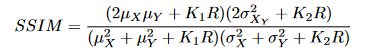
\includegraphics[width=0.60\linewidth]{Figuras/Estado\_del\_Arte/Stegomalware/SSIM.png}
  \label{fig:SSIM}
  \caption{SSIM (\cite{stegomalware})}
\end{figure}

En general, los valores de las variables \textit{K1} y \textit{K2} serán de 0.01 y 0.03 respectivamente. Los resultados de \ac{SSIM} pueden variar desde -1 a 1, siendo el primero un indicativo de que las imágenes con esteganografía son más difíciles de identificar que las imágenes sin ésta. Para un buen algoritmo esteganográfico, lo mejor sería tener un valor bajo en esta métrica.

\subsubsection{EC}

La \ac{EC} es la relación del número total de bits embebidos en una imagen con el tamaño total de la imagen. También se la conoce como \ac{BPP}. Para una imagen con esteganografía con altura \textit{H}, anchura \textit{W}, y siendo el número de bits embebidos \textbf{E}, la \ac{EC} se representa como:

\begin{equation}
EC = \frac{E}{WH}
\end{equation}

\subsubsection{BPNZAC}

El \ac{BPNZAC} es el número de bits embebidos en los coeficientes \ac{DCT} de la imagen (\cite{dct}). Este número se selecciona para escoger la proporción de los bits embebidos, y es usado para evaluar el rendimiento. Dicho de otra forma, esta métrica es el equivalente al \ac{EC} en imágenes con formato JPEG. %cita

\subsubsection{QF}

El \ac{QF} es la métrica usada para medir la calidad de una imagen tras la compresión JPEG. Suele usarse tanto en el ámbito de la esteganografía en imágenes como en el estegoanálisis de imágenes JPEG. Se representa en forma de porcentaje y suele rondar entre el 75\% y el 100\%.

\subsubsection{PE}

La \ac{PE}, también conocida como \ac{DER}, de un método de estegoanálisis en imágenes es el número total promedio de imágenes con y sin esteganografía mal identificadas. Es decir, es el número promedio de falsos positivos y falsos negativos que hay. Se representa por la siguiente fórmula:

\begin{equation}
P_E = \frac{1}{2}(P_{F_A} + P_{M_D})
\end{equation}

\textit{$P_{F_A}$} es la probabilidad de falsa alarma, la cual indica la probabilidad de que las imágenes normales se clasifiquen como imágenes con esteganografía; y \textit{$P_{M_D}$} es la probabilidad de detecciones fallidas, la cual indica la probabilidad de que se hayan clasificado erróneamente las imágenes con esteganografía como imágenes normales. Esta métrica es usada principalmente para evaluar en sistemas de Machine Learning (y de Deep Learning) técnicas de estegoanálisis en imágenes para detectar información oculta.

\subsubsection{DA}

La \ac{DA} es otra métrica usada comúnmente en este ámbito de evaluación de rendimiento en estegoanálisis y esteganografía, ya que mide la relación entre el número total de clasificaciones correctas entre imágenes con y sin esteganografía, dividida por el número total de clasificaciones correctas e incorrectas para ambos tipos de imágenes. Esta fórmula se representa de la siguiente forma:

\begin{equation}
Detection Accuracy (DA) = \frac{TP + TN}{TP + TN + FP + FN}
\end{equation}

Donde \textit{TP} son el número de clasificaciones correctas para imágenes con esteganografía, \textit{TN} son el número de clasificaciones correctas para imágenes normales, \textit{FP} son el número de falsos positivos (clasificaciones incorrectas de las imágenes normales) y \textit{FN} son el número de falsos negativos (clasificaciones incorrectas de las imágenes con esteganografía).

Alternativamente, podemos representar con la siguiente ecuación la \ac{PE}, ya que la suma de ambas métricas siempre da 1:

\begin{equation}
Probability of error (P_E) = 1 - DA
\end{equation}

\subsubsection{BER}

La \ac{BER} cuantifica la robustez de los datos embebidos en la imagen. Sea un algoritmo de esteganografía en el que \textit{B} es el número de bits embebidos en la imagen y \textit{BE} es el número de errores ocurridos durante la extracción de los datos embebidos, la ac{BER} se representa como:

\begin{equation}
BER = \frac{B_E}{B}
\end{equation}

\subsubsection{MAE}

El \ac{MAE} se identifica como el promedio del valor absoluto de los errores. El error absoluto es el valor absoluto de la diferencia entre los valores predichos y los valores reales. Se representa mediante la siguiente figura:

\begin{figure}[H]
  \centering
  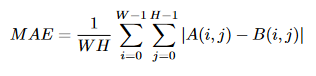
\includegraphics[width=0.45\linewidth]{Figuras/Estado\_del\_Arte/Stegomalware/MAE.png}
  \label{fig:MAE}
  \caption{MAE (\cite{stegomalware})}
\end{figure}

Siendo \textit{A} y \textit{B} dos imágenes monocromáticas con una anchura \textit{W} y una altura \textit{H}.

El \ac{MAE} puede ser usado para medir la calidad de una imagen con esteganografía comparada con una imagen normal.

\subsubsection{QI}

El \ac{QI} es la medida de la distorsión de la imagen usando factores como la pérdida de correlación, la distorsión de luminancia y la distorsión de contraste. Se puede representar por la siguiente fórmula:

\begin{figure}[H]
  \centering
  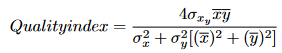
\includegraphics[width=0.45\linewidth]{Figuras/Estado\_del\_Arte/Stegomalware/QI.png}
  \label{fig:QI}
  \caption{QI (\cite{stegomalware})}
\end{figure}

La \textit{x} y \textit{y} son las imágenes normales y con esteganografía respectivamente, y la media y la varianza de los valores de los píxeles de éstas se representan como \textit{$\bar{x}$}, \textit{$x^{2}$} y \textit{$\bar{y}$}, \textit{$y^{2}$} (\cite{qi}).%#cita

\subsubsection{Conclusión}

Dentro de todas las posibilidades vistas, y de forma convencional, las métricas usadas en la evaluación de rendimiento para estegoanálisis en imágenes suelen ser \ac{DER} y \ac{DA}. Cuando llegue el momento de realizar los experimentos las tendremos en cuenta.

\section{MalJPEG}

En este proyecto se trata una solución basada en Machine Learning para detectar imágenes JPEG maliciosas. Al igual que con Stegomalware primero veremos cómo es la solución propuesta por los autores y bajo qué condiciones puede actuar, seguido de las métricas utilizadas para sus experimentos.

\subsection{Contexto}

Durante mucho tiempo, los archivos con formato JPEG han sido unos de los más utilizados tanto en el ámbito empresarial como en el del individuo. En gran parte ha sido gracias a su compresión con pérdidas basada en \ac{DCT}, y es por ello que se han convertido rápidamente en un atractivo vector de ataque para los cibercriminales. Para ello, la solución que se propone en este artículo se denomina \textbf{MalJPEG}, y su objetivo no es otro que saber clasificar correctamente si una imagen JPEG es maliciosa o no, mediante tecnología basada en Machine Learning.

\subsection{Solución}

El funcionamiento de MalJPEG se basa en extraer estadísticamente, es decir, sin mirar la imagen como tal, características del archivo (por ejemplo, el tamaño del archivo en bytes). Después se aplican diferentes algoritmos de Machine Learning que tomarán como entrada dichos datos, y clasificarán las imágenes como maliciosas o benignas; tal y como viene en la imagen:

\begin{figure}[H]
  \centering
  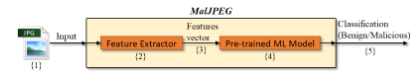
\includegraphics[width=0.75\linewidth]{Figuras/Estado\_del\_Arte/MalJPEG.png}
  \label{fig:MalJPEG}
  \caption{Esquema de MalJPEG (\cite{maljpeg})}
\end{figure}

\subsubsection{Métodos genéricos de extracción de características}

Generalmente existen dos métodos de extracción de características que, en este artículo, se utilizan: los que están basados en \textbf{histogramas} y la técnica \textbf{Min-Hash}. A continuación, pasamos a explicarlos brevemente:

\begin{itemize}
\item \textbf{Histogramas}
\begin{itemize}
\item Los métodos de extracción basados en histogramas crean un histograma en el que se recogen datos y valores propios del archivo en cuestión, para poder utilizarlos como entradas en algoritmos de Machine Learning. En este artículo, se han usado dos tipos de histogramas: \textbf{histogramas simples} e \textbf{histogramas de entropía de bytes avanzados}.
\item Para los primeros se usan 2 configuraciones: histogramas basados en valores de bytes e histogramas basados en valores de caracteres. El histograma cuenta la frecuencia de estos valores en el archivo para cada configuración. Para poder comparar archivos con diferente tamaño es necesario normalizar los valores de los histogramas entre 0 y 1.
\item Para los segundos, se desliza una ventana de bytes de tamaño \textit{K}, con un salto de \textit{S} bytes, sobre la representación en bytes del archivo. Para cada ventana, calculamos la entropía en base 2 del archivo (\textbf{véase la siguiente figura}). Guardamos cada valor individual de los bytes en la ventana con el valor de la entropía de toda la ventana (en pares) en una lista; de este modo, habrá \textit{K} pares por cada ventana. Por último, calculamos un histograma en 2 dimensiones con un eje \textit{E} que representará la entropía, y un eje \textit{B} que representarán los bytes. En este punto es donde se obtiene el vector de características de la imagen basado en el histograma.

\begin{figure}[H]
  \centering
  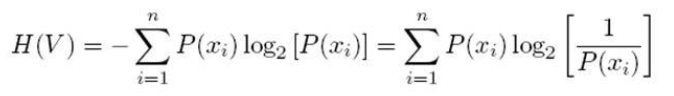
\includegraphics[width=0.75\linewidth]{Figuras/Estado\_del\_Arte/Entropia.png}
  \label{fig:entropia}
  \caption{Fórmula de la entropía (\cite{entropia})}
\end{figure}

\end{itemize}
\item \textbf{Min-Hash}
\begin{itemize}
\item Esta técnica se basa en estimar rápidamente cómo de similares son dos objetos. El método Min-Hash genera una firma de tamaño \textit{N} para un archivo dado basada en \textit{N} simples funciones hash (\cite{min-hash}). Después se calcula la distancia de Hamming entre las firmas de los dos objetos a comparar: cuanto más pequeña la distancia, más coincidencias en las firmas (\cite{hamming}). %cita
\item La firma de Min-Hash se basa en \textit{shingles} extraídas del archivo. Un shingle es una secuencia de longitud fija con unidades básicas del archivo (bytes, caracteres, entre otras). Cada shingle se extrae mediante una ventana de tamaño \textit{W} con un salto de \textit{S} bytes por todo el archivo (como las ventanas de tamaño \textit{K} en los histogramas basados en entropía de bytes). Se aplican \textit{N} funciones hash en cada shingle extraído, y los resultados de los hashes se guardan en un vector de tamaño \textit{N}.
\item Finalmente, se consigue la firma, la cual es un vector de tamaño \textit{N} que contiene el mínimo valor de hash producido por cada función hash, a través de todos los shingles.
\end{itemize}
\end{itemize}

\subsubsection{Algoritmos de Machine Learning}

De cara a utilizar las características de la imagen como parámetros de entrada de la parte de Machine Learning de esta solución, los autores cotejaron varios tipos de algoritmos usados comúnmente en el ámbito de clasificación de imágenes. Dentro de estos tenemos:

\begin{itemize}
\item \textbf{Decision Tree}
\item \textbf{Random Forest}
\item \textbf{Gradient Boosting en Decision Tree (XGBoost y LightGBM)}
\end{itemize}

Por lo general, estos algoritmos de clasificación son muy apropiados para datasets con más cantidad de objetos de una clase que de otra. Por otro lado, en este artículo también se cotejó el clasificador \textbf{K-Nearest Neighbors} en los datasets de Min-Hash; ya que éste es el único capaz de comparar firmas de Min-Hash usando la función de la distancia de Hamming.

\subsubsection{Métricas}

Para evaluar la clasificación de las imágenes se han cogido métricas como la \ac{TPR} y la \ac{FPR} (derivadas presumiblemente de la \ac{DER}). Por otro lado, y considerando estas métricas podemos utilizar la \ac{ROC}: la \ac{ROC} es la curva creada en una gráfica entre los valores de la \ac{TPR} y la \ac{FPR} en diferentes umbrales. Teniendo la \ac{ROC} podemos medir la \ac{AUC}, es decir, el área bajo la curva de la \ac{ROC}; de este modo si el valor de la \ac{AUC} es alto, quiere decir que el valor de la \ac{TPR} también lo es, mientras que el valor de la \ac{FPR} es bajo (\cite{auc}). %cita

Sin embargo, no sólo se necesitan esas métricas. Hace falta una que optimice los resultados de la detección de los clasificadores, sirviéndose de la \ac{TPR} y la \ac{FPR}: la \ac{IDR} (\cite{idr}). %cita

\begin{equation}
IDR = TPR*(1 - FPR) = TPR*TNR
\end{equation}

La \ac{IDR} indica el punto del clasificador en el que se ha optimizado adecuadamente, y todo pasa por tener un valor muy alto en \ac{TPR} y uno muy bajo en \ac{FPR}. Cuanto mayor sea la \ac{IDR}, tendremos un mejor clasificador.

\section{ImageDetox}

Esta solución se creó con el objetivo de detectar y neutralizar código malicioso oculto en imágenes, aunque para ello no utilice tecnología de Machine Learning (\cite{imagedetox}). Sin embargo, es interesante comprobar en qué consiste y qué métricas decidieron utilizar los autores. %cita

\subsection{Solución}

ImageDetox es un método creado con el pretexto anterior incluso sin una información previa del código que se ha introducido. El método se compone de cuatro módulos:

\begin{itemize}
\item \textbf{Extracción del archivo de imagen}
\item \textbf{Análisis del formato del archivo de imagen}
\item \textbf{Conversión del archivo de imagen}
\item \textbf{Gestión del archivo de imagen tras la conversión}
\end{itemize}

La solución propuesta puede servir, además, para evitar amenazas de seguridad resultantes del escondite de información confidencial en archivos de imagen, con el objetivo de sacar a la luz dichas amenazas. El esquema de la propuesta es como se muestra en la figura:

\begin{figure}[H]
  \centering
  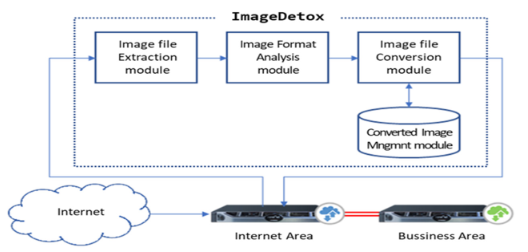
\includegraphics[width=0.75\linewidth]{Figuras/Estado\_del\_Arte/ImageDetox.png}
  \label{fig:ImageDetox}
  \caption{Esquema de ImageDetox (\cite{imagedetox})}
\end{figure}

De forma resumida, ImageDetox funciona de la siguiente manera:
\begin{enumerate}
\item  El primer módulo extrae los archivos de imagen de todos los archivos introducidos al área de Internet (la red local).
\item El segundo módulo identifica el formato de la imagen de la cabecera del archivo extraído en el paso anterior.
\item El tercer módulo aplica una conversión en la imagen con la que se consigue eliminar el código oculto (aun sin saber si tiene uno o no).
\item El cuarto módulo guarda el valor del hash de la imagen original en la imagen convertida, por un período de tiempo, una vez que se almacena en la unidad de gestión. El valor de los hashes de los archivos de imagen que han sobrepasado un cierto período de tiempo de almacenado, se borra del almacenamiento junto con el archivo de imagen, y la información se actualiza periódicamente según los futuros hashes que puedan llegar.
\end{enumerate}

\subsection{Métricas}

En este artículo no se utiliza ninguna de las métricas usadas en los otros modelos vistos, aquí se crean dos tipos de métricas únicas para esta solución: \textbf{VT Detection (A)} y \textbf{VT Detection (B)}.

VT Detection (A) hace referencia al número de antivirus que son capaces de detectar malware oculto en una imagen dividido entre el número de antivirus usados para detectar virus en una imagen. Dicho de otra forma, representa los resultados de analizar si cada imagen maliciosa original es maliciosa, según determina VirusTotal (\cite{virustotal}). %cita

Por el contrario, VT Detection (B) hace referencia al resultado de la detección después de utilizar esta técnica de neutralización propuesta en las imágenes con código malicioso. Dicho de otra forma, representa los resultados de analizar si cada imagen maliciosa original es maliciosa tras aplicar esta técnica.
